\documentclass[a4paper,12pt]{article}
\usepackage[utf8]{inputenc}
\usepackage{graphicx}
\usepackage[english]{babel}
\usepackage{geometry}
\usepackage{setspace}
\usepackage{minted}
\usepackage{booktabs}
\usepackage{amsmath}
\usepackage[table]{xcolor}
\usepackage{array}


\geometry{margin=1in}
\onehalfspacing

\begin{document}

\begin{titlepage}
    \begin{center}
        % adjust the logo here
        % Title
        {\Large \textbf{Genetic Data Analysis of Rheumatoid arthritis and Clouston's disease}} \\[1cm] 
        
        % Subtitle
        \textit{Module: M1 Méthodologie de traitement de données NGS} \\[3cm]
        

        \vfill % to push the authors to the bottom of the page

        \textbf{Authors} \\[0.5cm]
        \textsc{Ngoc VU, Denys BURYI}


    \end{center}
\end{titlepage}

\newpage


\section*{Introduction}

We have carried out linkage analyses (LOD score or affected sib-pairs) 
and association analyses (case-control or familial) for a monogenic disease, then for a multifactorial disease:
\begin{enumerate}
    \item Study of a monogenic disease: Clouston's disease
    \begin{enumerate}
        \item Genetic linkage analysis (LOD score)
        \item Familial association analysis
    \end{enumerate}
    \item Study of a multifactorial disease: rheumatoid arthritis
    \begin{enumerate}
        \item Genetic linkage analysis (affected sib-pairs)
        \item Genome-Wide case-control association analysis
    \end{enumerate}
\end{enumerate}

 
The data and programs were provided by our professor VALÉRIE CHAUDRU.

\section{Monogenic disease: Clouston's disease}

Clouston syndrome is mainly characterized by abnormal nails (thickened, slow-growing, brittle) 
and alopecia (hair loss). \textit{Palmoplantar hyperkeratosis} (commonly known as horniness) is 
also sometimes observed. 
This is a rare disease, with a prevalence ranging from 1 to 9 in 100,000. It is autosomal dominant. 
Penetrance of the disease is complete, but its expression is variable, even in patients from the same family.
Our aim in this part of the analysis was to:

\begin{itemize}
    \item Perform linkage analysis using the LOD score method to locate the Clouston disease gene 
    using genetic markers located on chromosome 13.
    \item Interpret data from a \texttt{.vcf} file containing genetic variants identified in a 
    case-control sample and perform association analysis for a candidate variant.
    \item Search for the causal genetic variant using familial association analysis.
\end{itemize}

\subsection{Genetic linkage analysis - LOD score method}

We have analyzed the data contained in the \texttt{fam.txt} file using \texttt{paramlink} package in R. 
First we performed some initial data exploration using \texttt{linkdat()} and \texttt{summary()} functions:

    
    \begin{minted}[frame=lines, linenos]{r}
        fam = read.table('fam.txt')
        x = linkdat(fam)
        summary(x)
        \end{minted}

We found that the file contains data of a large family of 47 individuals, comprising 22 affected and
 25 unaffected members. These individuals are organized into 10 nuclear subfamilies and 
have been genotyped for 13 genetic markers on chromosome 13. For 11 individuals in the dataset no 
parent data was available (further referred to as "founders"). Figure \ref{fig:pedigree} shows 
the pedigree plot of the family.

\begin{figure}[ht!] % ht! means here at the top, despite placing rules 
    \centering
    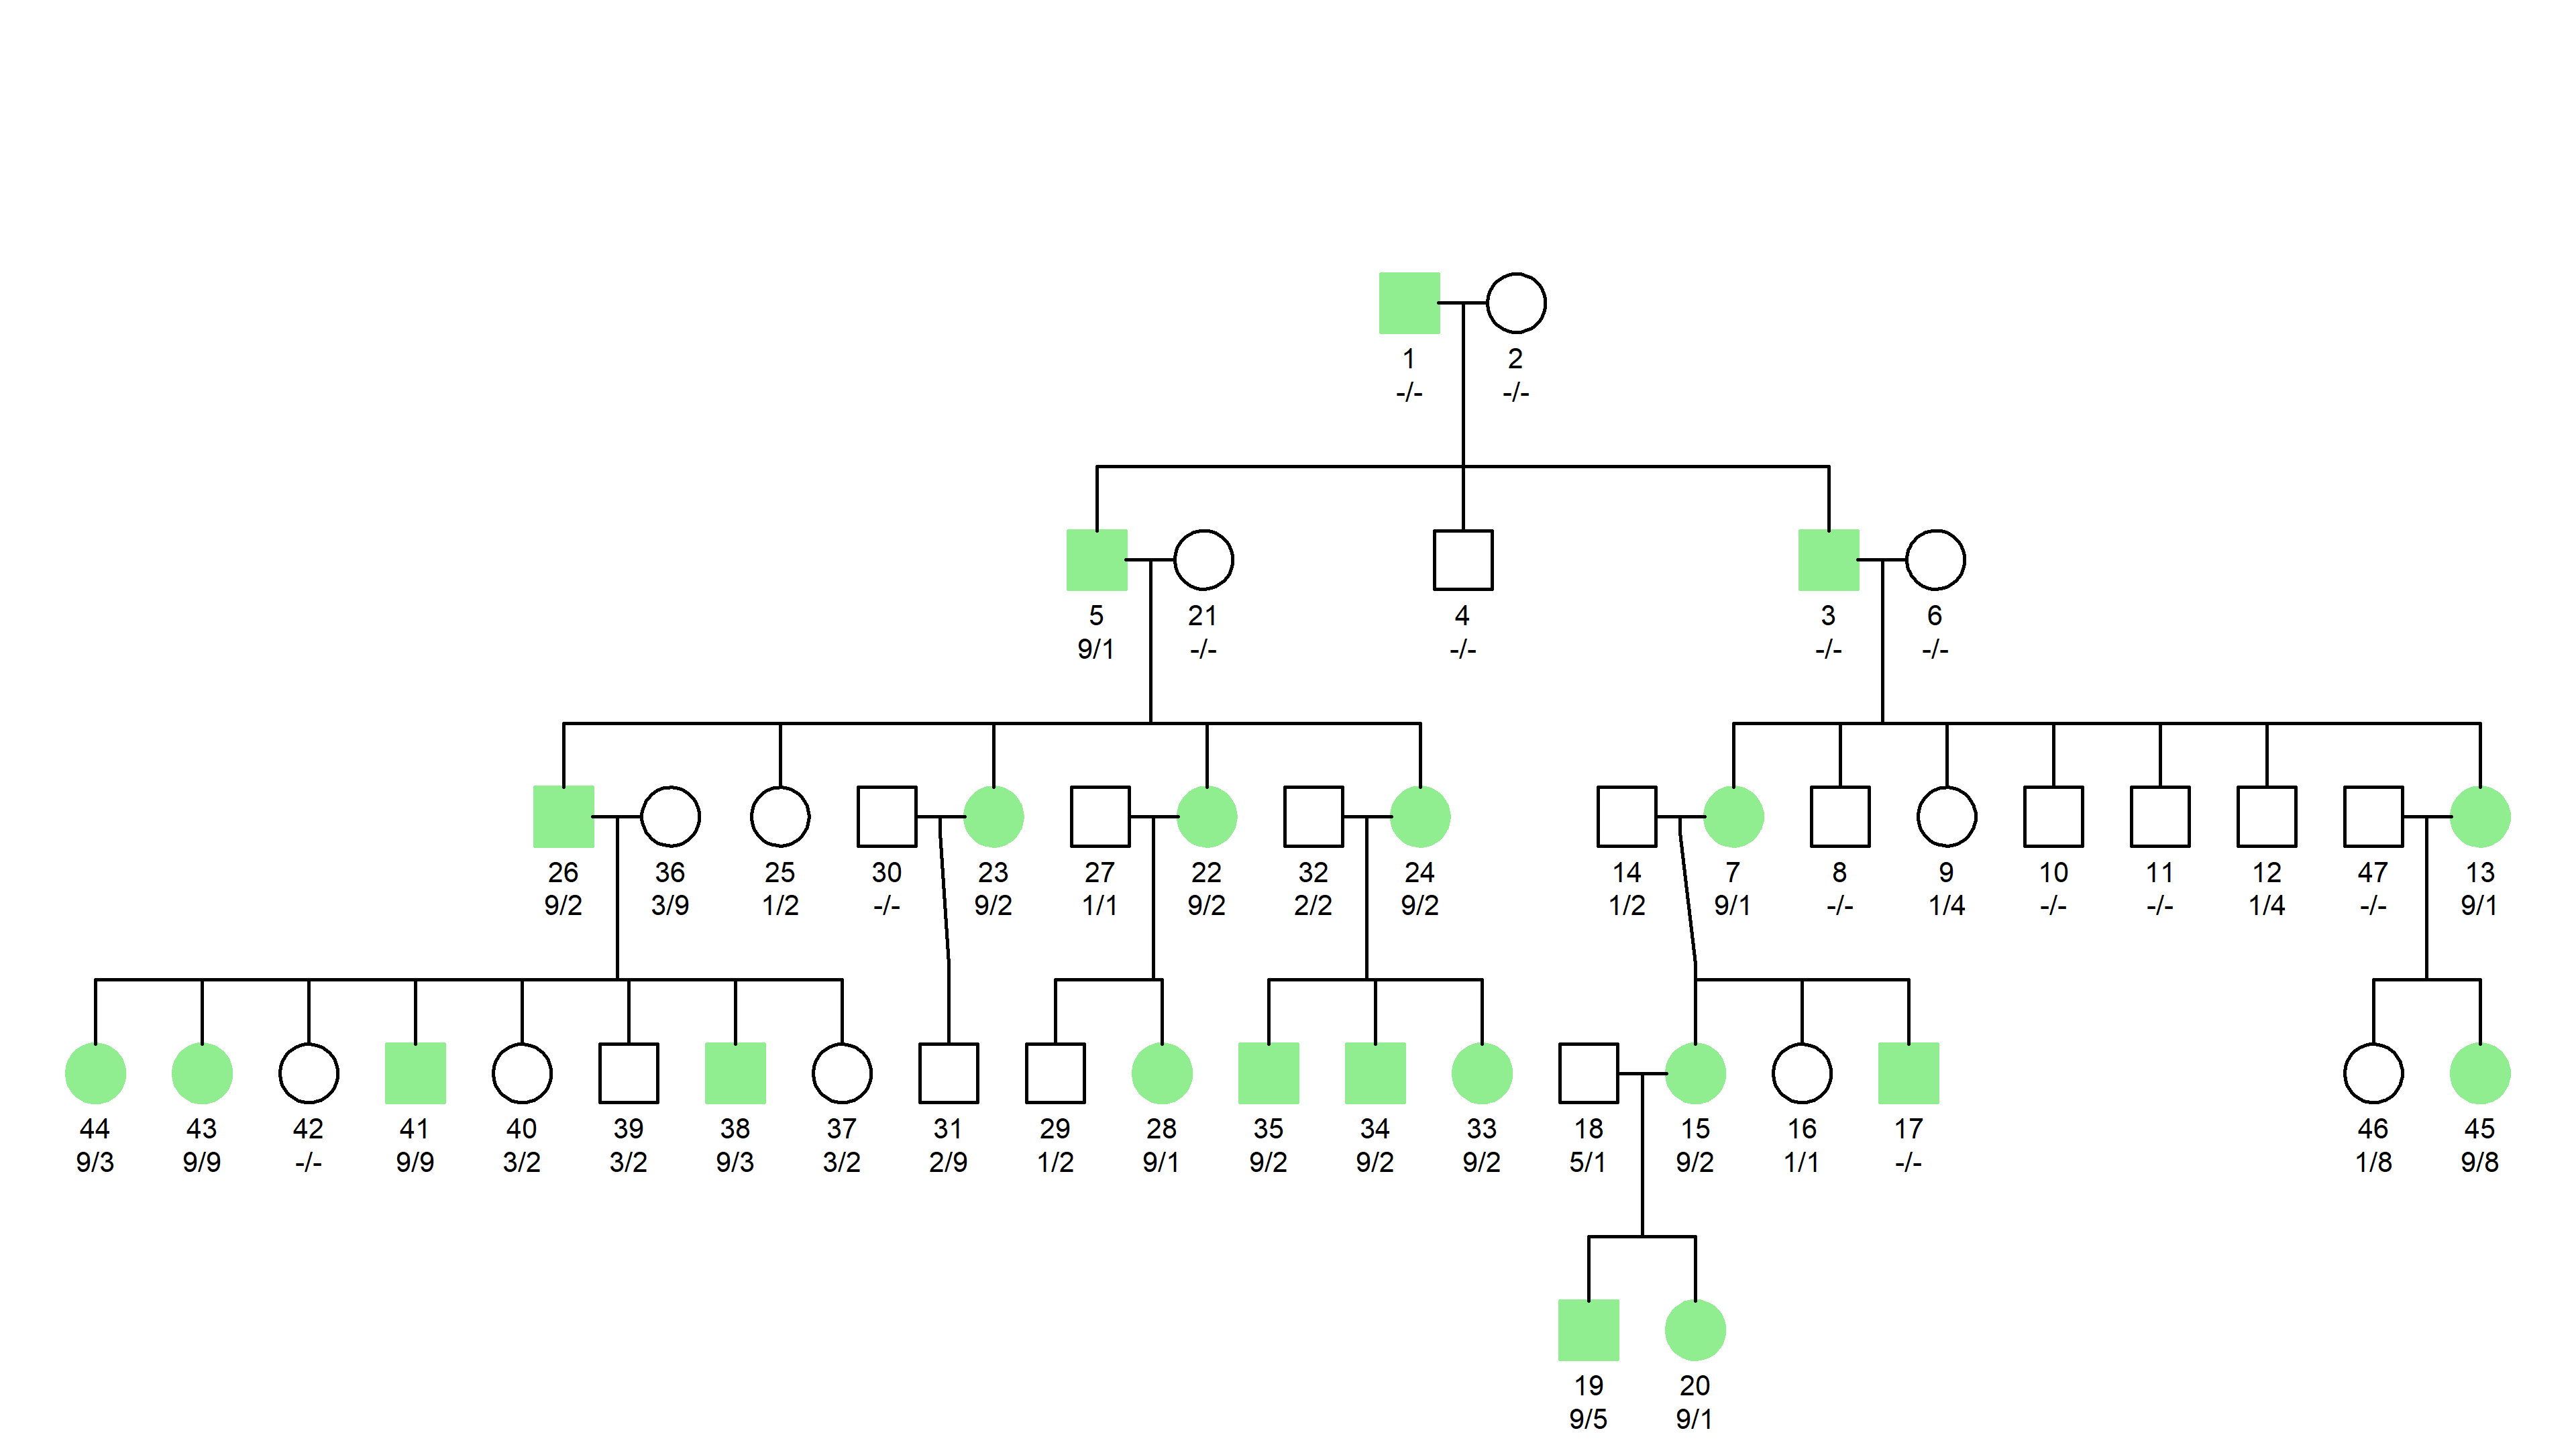
\includegraphics[width=\textwidth]{images/pedigree_plot.png}
    \caption{Pedigree plot of the family along with their affection status and genotypes with 
    regards to marker 1.
    Affected - light green, Unaffected - white. Sex: square/circle - M/F. Genotype: alleles of the marker 1.}
    \label{fig:pedigree} % this allows to reference the figure with \ref{fig:pedigree}

    
\end{figure}

In addition to helping summarize the data, the \texttt{linkdat()} function also transforms the original data
and outputs a \texttt{linkdat} object that can be used to perform linkage analysis. \texttt{linkdat} object 
is a list containing among others, the following important components:
\begin{itemize}
    \item \texttt{pedigree} - data.frame with 5 columns (ID, FID, MID, SEX, AFF) describing the pedigree in linkage format.
    \item \texttt{orig.ids} - vector of original IDs of the individuals in the pedigree.
    \item \texttt{subnucs} - list of vectors of IDs of individuals in each nuclear family.
    \item \texttt{markerdata} - a list of \texttt{marker} objects describing information about the genetic markers.
\item \texttt{model} - a list of parameters for the linkage analysis.
\end{itemize}



\subsection{Mode of inheritance: Autosomal Dominant}

First, we have analyzed our data assuming an autosomal dominant mode of inheritance. Using the \texttt{setmodel()} function,
we have set the parameters to:
\begin{itemize}
    \item phenocopies = $10^{-5}$
    \item complete penetrance
    \item disease allele frequency = $10^{-5}$
\end{itemize}

We then performed the linkage analysis using the \texttt{lod()} function for a range of $\theta$ from 0 to 0.5 with a step of 0.05. 
We have saved the results in the \texttt{result\_dom} data frame for further analysis (see code below).

\begin{minted}[frame=lines, linenos]{r}
    xdom = setModel(x, model=1, penetrances = c(0.00001, 1, 1), dfreq = 0.00001)
    result_dom = lod(xdom, theta=c(0, 0.05, 0.1, 0.15, 0.2, 0.25, 0.3, 0.4, 0.5)) 
    result__dom_df = as.data.frame(result_dom)
\end{minted}

\begin{figure}[hb!] % b for bottom 
    \centering
    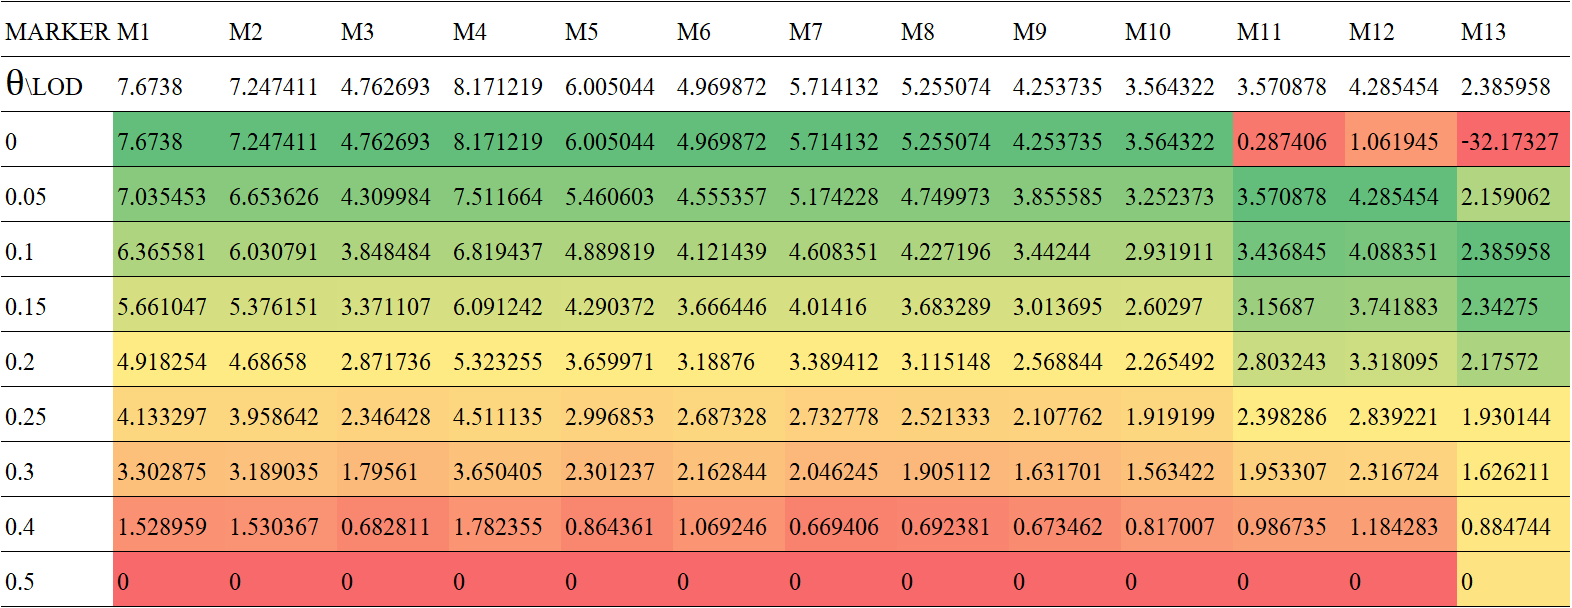
\includegraphics[width=\textwidth]{images/xdom_lod_analysis.png}
    \caption{LOD score analysis results for autosomal dominant mode of inheritance. Each column shows 
    LOD score for a given marker, for a given $\theta$ value. Top row shows maximum LOD score for each marker. 
    Conditional coloring: green to red - higest to lowest LOD score.}   
    \label{fig:xdom_lod_score} 
    
\end{figure}

When performing LOD score analysis, under the null hypothesis $\mathit{H_0}$ we assume 
that there is no linkage between the markers and the disease gene and $\mathit{\theta = 0.5}$. In other words if the two 
loci are unlinked, the probability of observing a recombinant event $\mathit{c = 50\%}$. Under an alternative
hypothesis $\mathit{H_1}$, if the two loci are indeed linked, we expect the probability of observing a recombinant 
event \textit{c} to fall within $0 < c < 50\%$. LOD score is a logarithmic likelihood ratio:

\[
\mathit{Z(x) = \log_{10} \left[ \frac{L(c = x)}{L(c = 0.5)} \right]}
\]
A LOD score of 3 indicates a 1,000:1 likelihood that two genes are linked and inherited together with a given 
recombination rate(e.g. \textit{c=10\%}), compared to the likelihood under the null hypothesis.
For all markers except M13, the maximum LOD score exceeds 3 (see Figure \ref{fig:xdom_lod_score}).
These results suggest that the disease gene is likely in extremely close proximity to markers 1–10, 
and approximately 5 cM away from markers 11 and 12.

As for marker 13, it is highly probable that adding more families to the dataset would increase $\mathit{Z(max)}$ 
above 3. For now, the data suggest that the disease gene might be located approximately 15 cM from marker 13.

To validate these findings, we performed the same analysis using $\theta$ values ranging from 0 to 0.05 in 
increments of 0.01 (see Figure \ref{fig:xdom_LOD_score_granular}).



\begin{figure}[t] % t for top 
    \centering
    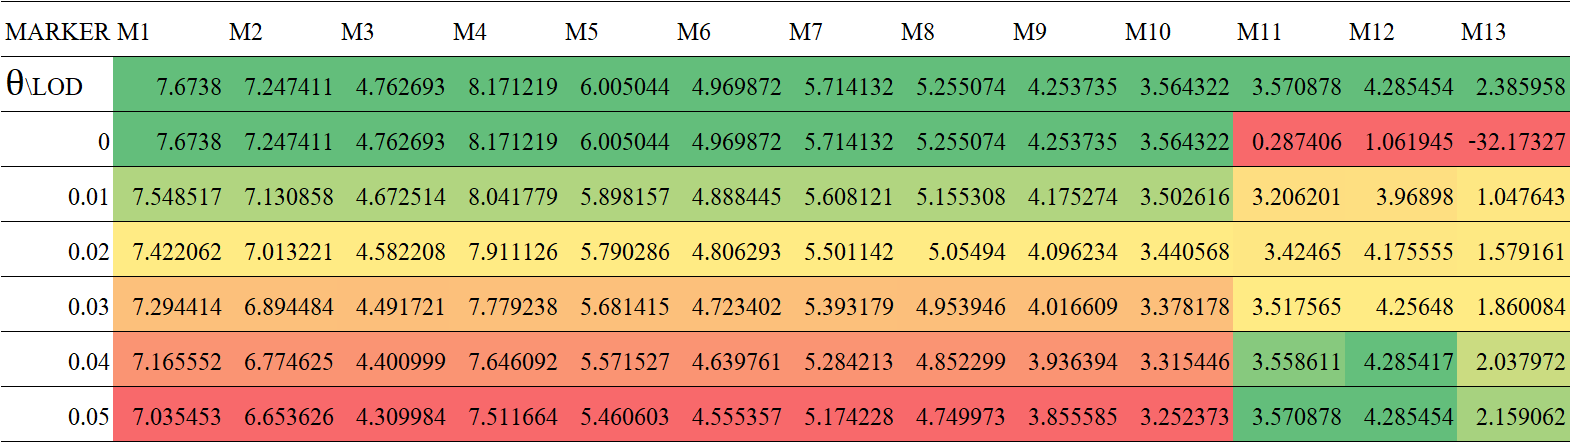
\includegraphics[width=\textwidth]{images/xdom_lod_analysis_more_granular.png}
    \caption{LOD score analysis results for autosomal dominant mode of inheritance for more 
    granular $\theta$ values. Each column shows LOD score for a given marker, for a given 
    $\theta$ value. Top row shows maximum LOD score for each marker. Conditional coloring: 
    green to red - highest to lowest LOD score.}   
    \label{fig:xdom_LOD_score_granular} 
    
\end{figure}

Next, we calculated the confidence intervals for each marker. % explanation here of why Zmax - 1 
Visualizing the LOD score curve can be helpful for this purpose, so we plotted it for marker 1 as 
a representative example for markers 2\-10 (Figure \ref{fig:lod_curve}). 
To determine the precise confidence intervals for the results as well as more precise 
$\mathit{Z_{max}}$ and $\mathit{\theta_{Zmax}}$, we ran the script located in 
the \texttt{ci\_bounds.R} file. Results are shown in the Table \ref{tab:ci_bounds}.

\begin{figure}[ht!] % t for top 
    \centering
    \includegraphics[width=\textwidth]{images/LOD-score_curve_M1.png}
    \caption{LOD score curve for marker 1. LOD score values on the y-axis, $\theta$ values on the x-axis. 
    Grey line represents the $\mathit{Z_{max}-1}$ value.}  
    \label{fig:lod_curve} 
    
\end{figure}

\begin{table}[ht!]
    \centering
    \begin{tabular}{ccccc}
        \toprule
        \textbf{Marker} & \textbf{$\mathit{\theta_{Zmax}}$} & \textbf{$\mathit{Z_{max}}$} & \textbf{Lower} & \textbf{Upper} \\ 
        \midrule
        1 & 0.000 & 7.6738 & 0.000 & 0.077 \\ 
        2 & 0.000 & 7.2474 & 0.000 & 0.082 \\ 
        3 & 0.000 & 4.7627 & 0.000 & 0.109 \\ 
        4 & 0.000 & 8.1712 & 0.000 & 0.074 \\ 
        5 & 0.000 & 6.0050 & 0.000 & 0.090 \\ 
        6 & 0.000 & 4.9699 & 0.000 & 0.116 \\ 
        7 & 0.000 & 5.7141 & 0.000 & 0.090 \\ 
        8 & 0.000 & 5.2551 & 0.000 & 0.097 \\ 
        9 & 0.000 & 4.2537 & 0.000 & 0.122 \\ 
        10 & 0.000 & 3.5643 & 0.000 & 0.089 \\ 
        11 & 0.051 & 3.5710 & 0.019 & 0.201 \\ 
        12 & 0.045 & 4.2882 & 0.019 & 0.201 \\ 
        13 & 0.111 & 2.3914 & NA & NA \\ 
        \bottomrule
    \end{tabular}
    \caption{Confidence intervals for each marker, including the maximum LOD score ($\mathit{Z_{max}}$) 
    and the corresponding recombination fraction ($\mathit{\theta_{Zmax}}$). For marker 13, results are inconclusive.}
    \label{tab:ci_bounds}
\end{table}

\subsection{Allele frequencies and LOD score}

So far in our analysis we have assumed that marker allele frequencies(AF) in the general population 
are equal, which isn't always true. If one of the alleles has a higher AF, it will have 
implication for the LOD score.
The reason changing AF influences the LOD score is because of the way genotypes are estimated for 
founders in the sample. If every allele is equally likely, the probability for each 
genotype (assuming 4 alleles) is: 
$\mathit{0.25 * 0.25 = 0.0625 \ or \ 6.25\%}$ for each. 

But let's assume that for alleles 1-4 if known allele frequencies are 0.1, 0.1, 0,1 and 0.7 respecivelly. 
In this case the probabilities of occurence for genotypes 4/4 and 1/4 are: 
\[
\text{Genotype } 4/4 \;=\; 0.7 \times 0.7 \;=\; 0.49 \;=\; 49\%
\]
\[
\text{Genotype } 1/4 \;=\; 0.1 \times 0.7 \;=\; 0.07 \;=\; 7\%.
\]

This has implications on LOD score when considering founders in the sample. When you change the allele 
frequencies for a marker, you alter the prior probabilities of founder genotypes, since founders rely 
on these frequencies to estimate their most likely alleles. This shifts the overall likelihood of 
observing the pedigree data under each hypothesis (linked vs.\ unlinked). Formally, the LOD score 
is defined as the base-10 logarithm of the ratio of the pedigree likelihood under the linked hypothesis 
to that under the unlinked hypothesis:
\[
\mathrm{LOD} \;=\; \log_{10} \Bigl(
  \frac{P(\text{data} \mid \theta < 0.5)}{P(\text{data} \mid \theta = 0.5)}
\Bigr).
\]
Since updated allele frequencies can either make the observed genotypes more plausible under linkage 
or under no linkage, the resulting LOD score can go up or down depending on whether these new priors 
improve the fit of the data more for the linked model than for the unlinked model (or vice versa).

Next we have performed the same analysis as above for just marker 5, with the updated allele frequencies 
for it's 4 alleles(0.1, 0.1, 0,1 and 0.7). Considering previous results have shown that linkage between 
marker 5 and the disease gene is likely, we expect the LOD score to increase, which was confirmed 
by our results (see Table \ref{tab:lod_comparison}).


\begin{table}[ht]
    \centering
    \begin{tabular}{c|>{\columncolor[HTML]{DFF2D8}}c|>{\columncolor[HTML]{FDEDE4}}c}
        \hline
        \rowcolor{white} \textbf{$\theta$} & \textbf{LOD-mod AF} & \textbf{LOD-equal AF} \\ \hline
        0.0  & 6.1601 & 6.0050 \\ 
        0.05 & 5.6090 & 5.4606 \\ 
        0.1  & 5.0311 & 4.8898 \\ 
        0.15 & 4.4243 & 4.2904 \\ 
        0.2  & 3.7862 & 3.6600 \\ 
        0.25 & 3.1152 & 2.9969 \\ 
        0.3  & 2.4110 & 2.3012 \\ 
        0.4  & 0.9454 & 0.8644 \\ 
        \rowcolor{white} 0.5  & 0.0000 & 0.0000 \\ 
        \hline
    \end{tabular}
    \caption{LOD score comparison between data with modified and default allele frequencies for 
    different $\theta$ values. The left column remains uncolored, while the other two columns are colored to highlight differences. The first row with headers is explicitly white.}
    \label{tab:lod_comparison}
\end{table}

\subsection{Misspecifying the genetic model}

To demonstrate the impact of misspecifying the genetic model on the LOD score, we performed a linkage analysis 
on the same dataset, assuming an autosomal recessive mode of transmission while keeping the other parameters identical:
\begin{itemize}
    \item phenocopies = $10^{-5}$
    \item complete penetrance
    \item disease allele frequency = $10^{-5}$
\end{itemize}

Based on the results shown in Figure \ref{fig:xrec_lod}, we were unable to reject the null hypothesis (no linkage) 
for any marker at any $\theta$, as none of the LOD scores exceeded 3. For marker 9
maximum LOD score is 1.4 at $\theta = 0$, which could suggest possible linkage if more families 
were added to the dataset. But for the other markers that are very close to the disease gene based on previous 
results, the LOD scores are actually the lowest at $\theta = 0$.
This outcome aligns with expectations, given the prior knowledge of autosomal 
dominant mode of inheritance of the disease. This analysis shows the danger of misspecifying the mode of inheritance 
of the disease.
\begin{figure}
    \centering
    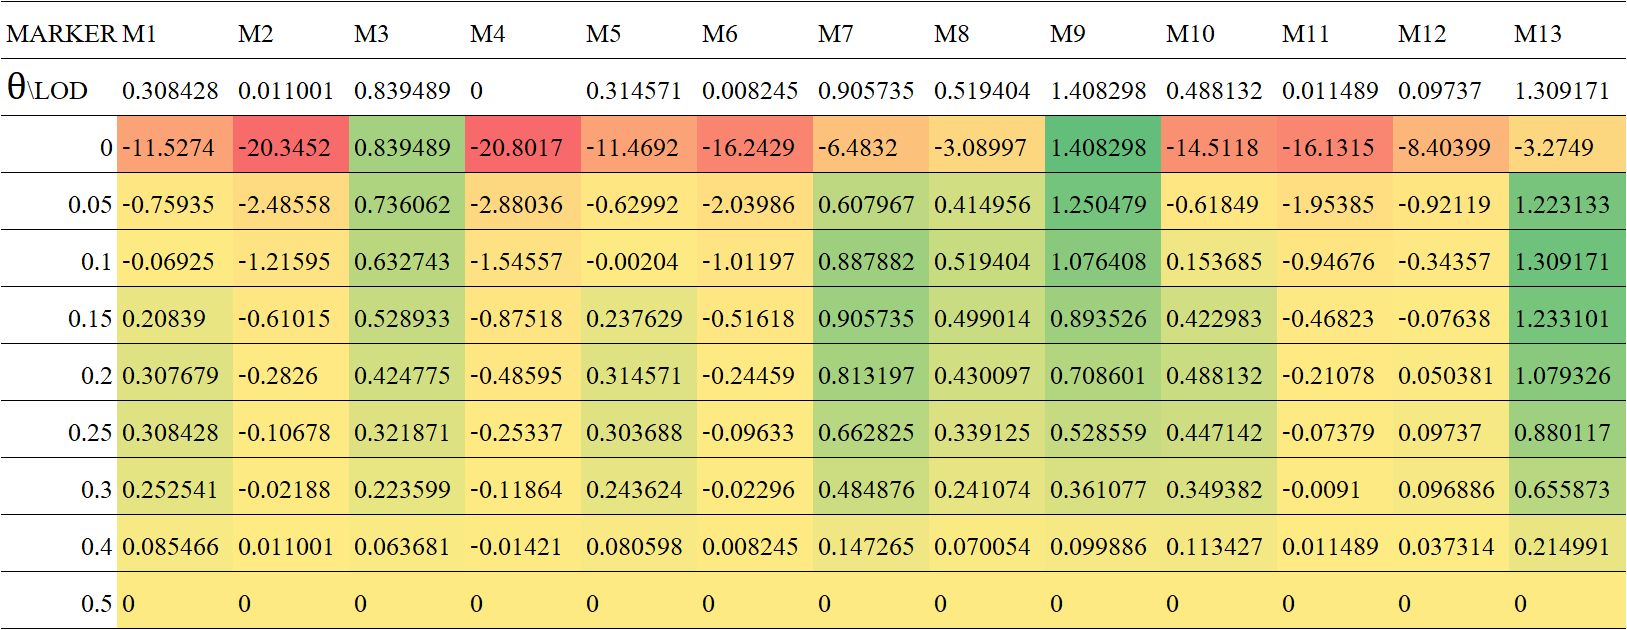
\includegraphics[width=\textwidth]{images/xrec_lod.png}
    \caption{LOD score analysis results for autosomal recessive mode of inheritance. Top row shows 
    maximum LOD score for each marker. Conditional coloring: green to red - higest to lowest LOD score.}
    \label{fig:xrec_lod}

\end{figure}


\section{Familial association analysis}

The gene GJB6 is situated within the linkage region identified in the previous section and appears to be a strong 
candidate for a driver gene. To investigate further, we conducted a familial association analysis using data from 
652 nuclear families, with an average of 3.1 individuals per family, genotyped for six SNP markers within the gene. 
We used \texttt{fbat.exe} program to analyze the data, with the following parameters:
\begin{itemize}
    \item \textbf{Trait: affection} \\
    Specifies that the test is focused on a affection status (e.g., affected vs. unaffected).
    
    \item \textbf{Offset: 0.000} \\
    The offset defines an adjustment for the null hypothesis. An offset of \texttt{0.000} assumes no deviation from 
    the null expectation in the absence of association.
    
    \item \textbf{Model: additive} \\
    The additive model assumes that the genetic effect of the allele increases additively with the number of copies 
    of the allele (e.g., heterozygotes have an intermediate effect between homozygotes for the major and minor alleles).
    
    \item \textbf{Test: bi-allelic} \\
    Specifies that the test is performed on bi-allelic markers (e.g., SNPs), considering only two alleles per locus.
    
    \item \textbf{Min family size: 10} \\
    Results are given for SNPs with at least 10 informative families.
    
    \item \textbf{Minimum allele frequency: 0.000} \\
    No exclusion based on allele frequency.
    
    \item \textbf{p-value threshold: 1.000} \\
    All p-values are reported, regardless of significance.
    
    \item \textbf{Maximum CMH statistic: 1000} \\
    Defines the upper limit for the Cochran-Mantel-Haenszel (CMH) statistic.
\end{itemize}

An informative family is one where at least one parent is heterozygous for the marker in question. Such families contribute 
to the analysis because heterozygosity allows the transmission of alleles to offspring to depend on the recombination rate. 
In contrast, families where parents are homozygous for the marker cannot provide information about linkage, as the likelihood 
of transmission does not vary with recombination.
The results are shown in the Table \ref{tab:fbat_results} below.

\begin{table}[ht]
    \centering
    \begin{tabular}{cccccccc}
        \toprule
        \textbf{Marker} & \textbf{Allele} & \textbf{afreq} & \textbf{fam\#} & \textbf{S-E(S)} & \textbf{Var(S)} & \textbf{Z} & \textbf{P} \\ 
        \midrule
        SNP2 & 1 & 0.636 & 409 & 3.500  & 138.750 &  0.297 & 0.766365 \\ 
        SNP2 & 2 & 0.364 & 409 & -3.500 & 138.750 & -0.297 & 0.766365 \\ 
        SNP3 & 1 & 0.370 & 402 & 2.000  & 140.500 &  0.169 & 0.866009 \\ 
        SNP3 & 2 & 0.630 & 402 & -2.000 & 140.500 & -0.169 & 0.866009 \\ 
        SNP4 & 1 & 0.403 & 425 & 5.000  & 148.500 &  0.410 & 0.681582 \\ 
        SNP4 & 2 & 0.597 & 425 & -5.000 & 148.500 & -0.410 & 0.681582 \\ 
        SNP5 & 1 & 0.626 & 393 & -4.500 & 136.750 & -0.385 & 0.700377 \\ 
        SNP5 & 2 & 0.374 & 393 & 4.500  & 136.750 &  0.385 & 0.700377 \\ 
        SNP6 & 1 & 0.212 & 283 & -52.000 & 91.000 & -5.451 & 5.01e-8 \\ 
        SNP6 & 2 & 0.788 & 283 & 52.000  & 91.000 &  5.451 & 5.01e-8 \\ 
        \bottomrule
    \end{tabular}
    \caption{Results of the FBAT analysis for SNPs with at least 10 informative families. Each SNP has two rows of results, 
    one for each allele. The columns are defined as follows: \textbf{Afreq} represents the allelic frequency, \textbf{Fam\#} 
    is the number of informative families, \textbf{S-E(S)} is the score used to test association minus its expected value 
    under the null hypothesis (with the sign indicating whether an allele is more or less frequently transmitted from 
    heterozygous parents to affected children), \textbf{Var(S)} is the variance of the score, \textbf{Z} is the test statistic 
    calculated as $(S-E(S))/\sqrt{Var(S)}$, and \textbf{P} is the p-value associated with the test ($p \leq 0.05$ indicates 
    rejection of $\mathit{H_0}$).}
    \label{tab:fbat_results}
\end{table}

SNP1 is not present in the above results since it didn't fulfill the criteria of having at least 10 informative families. 
For the rest of the SNPs no significant association was found, with once exception being SNP6. This SNP showed very high \textbf{S-E(S)} 
score with very high level of significance. Based on this score and its sign for the two alleles, we can say that allele 2 is transmitted from 
heterozygous parents to affected children much more frequently than allele 1. This suggests that allele 2 might be associated with 
the disease.
We then explored linkage disequilibrium (LD) between this SNP and other SNPs using Ensembl. We used GRCh37 version of human genome and the 
population of \texttt{1000GENOMES:phase\_3:CEU} since they are appropriate for the data we have. On the Figure \ref{fig:ld_plot} we 
can see teh result of our search. There are no SNPs in high LD with SNP6, which suggests that the association is not due to another nearby 
variant, but rather to SNP6 itself.

\begin{figure}[ht]
    \centering
    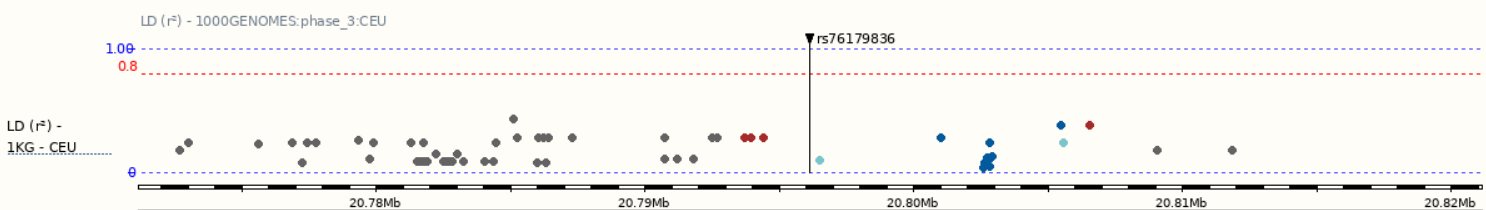
\includegraphics[width=\textwidth]{images/fbat_Ensembl_thin.png}
    \caption{Linkage disequilibrium plot for SNP6 - rs76179836 and other SNPs in the GJB6 gene. The plot shows the r2 values for 
    each pair of SNPs. On the x-axis shown are $\mathtt{r^2}$ values for each SNP. The blue and red dashed lines represent $\mathtt{r^2}$ of 1 
    and 0.8, respectively. On the y-axis are the coordinates on the chromosome.}
    \label{fig:ld_plot}
\end{figure}

\newpage
    \section{Multifactorial disease: Rheumatoid Arthritis}

\end{document}